%---------------Preamble---------------------
\documentclass{beamer}

% Theme and color
\usetheme{Madrid}
%\usetheme{Pittsburgh}
\usefonttheme{serif}
%\usecolortheme{default}
\usecolortheme{seahorse}
\setbeamertemplate{itemize items}[ball]

% Addtional Packages
\usepackage{listings}
\usepackage{algorithm}
\usepackage{algpseudocode}
\usepackage{xcolor}
\usepackage{caption} % captions in tables
\usepackage{graphicx} % images

% Styling python code globally
\lstdefinestyle{pythonstyle}{
  language=Python,
  backgroundcolor=\color{white},
  commentstyle=\color{green!40!black},
  keywordstyle=\color{blue},
  numberstyle=\tiny\color{gray},
  stringstyle=\color{purple!60!black},
  basicstyle=\ttfamily\footnotesize,
  breakatwhitespace=false,
  breaklines=true,
  captionpos=b,
  keepspaces=true,
  numbers=left,
  numbersep=5pt,
  showspaces=false,
  showstringspaces=false,
  showtabs=false,
  tabsize=2
}
\lstset{style=pythonstyle}

% Title details
\title{Reinforcement Learning for Pseudo-Labeling}
\subtitle{Capstone Project Presentation}
\author{
  Group-11
  \\
  \vspace{0.3cm}
  \textbf{Students:} Aishwarya Maddula, Deepika Reddygari, Phanindra Kalaga, Prudhvi Chekuri
  \\
  \vspace{0.3cm}
  \textbf{Guided by:} Dr. Amir Jafari, Prof. Tyler Wallett
}
\institute{George Washington University}
\date{}
%\date{\today}

% Footer Details
\setbeamertemplate{footline}{
  \leavevmode
  \makebox[\linewidth]{%
    \hspace{0.5cm}%
    \scriptsize \insertshorttitle%
    \hfill%
    \scriptsize \insertframenumber/\inserttotalframenumber \hspace{0cm}%
  }%
  \vspace{0.2cm}
}
%---------------Document---------------------

\begin{document}

%--------------------------

\begin{frame}
  \titlepage
\end{frame}

%--------------------------

\begin{frame}{Outline}
  \tableofcontents
\end{frame}

%--------------------------

\section{Introduction}
\begin{frame}{Introduction}
  \begin{itemize}
    \item \textbf{Problem:} Labeled data is limited and costly to obtain.
      %Labeled data is often scarce, and manual annotation is expensive and time-intensive.
      \\~\\
    \item \textbf{Challenge:} Traditional pseudo-labeling often propogates errors.
      %Conventional pseudo-labeling methods risk error propagation, degrading model performance.
      \\~\\
    \item \textbf{Idea:} Use Reinforcement Learning (RL) to adaptively select pseudo-labels and improve error rate.
      %Employ Reinforcement Learning (RL) to develop an adaptive pseudo-labeling strategy that optimizes sample selection and enhances model accuracy.
  \end{itemize}
\end{frame}

%--------------------------

\section{Background and Literature Review}
\begin{frame}{Background and Literature Review}
  \begin{itemize}
    \item The team began with introductory RL implementations using examples from the \texttt{gymnasium} library to build foundational understanding. \\~\\
    \item Conducted an initial review and implementation of five RL-based pseudo-labeling studies to establish a research baseline. \\~\\ \\~\\
      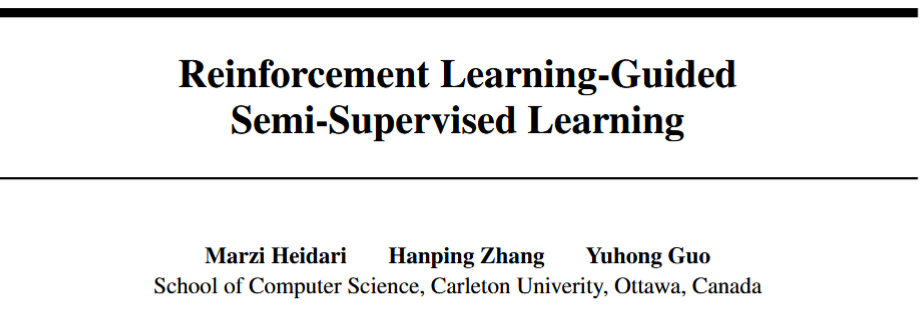
\includegraphics[width=0.32\linewidth]{RLPL/images/RLGSSL.png}
      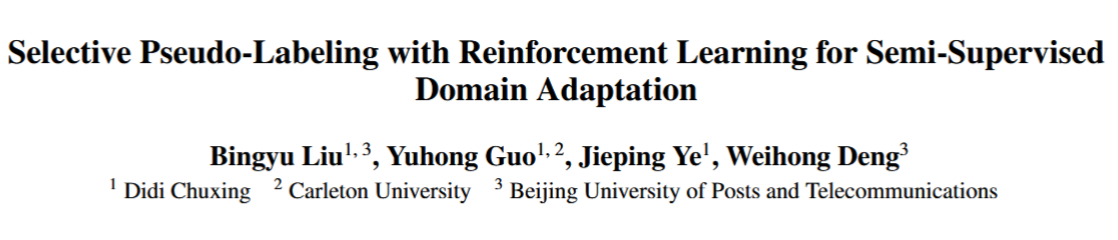
\includegraphics[width=0.32\linewidth]{RLPL/images/2012-03438.png}
      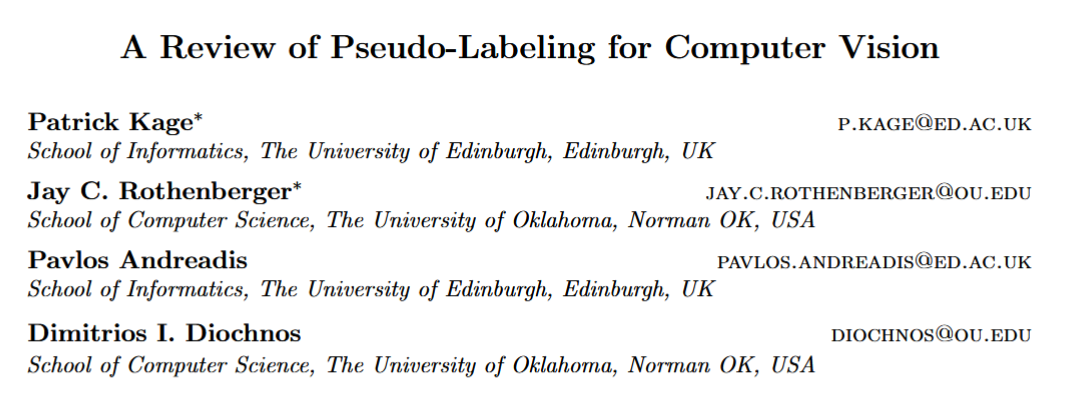
\includegraphics[width=0.32\linewidth]{RLPL/images/2408-07221.png}

  \end{itemize}
\end{frame}

%--------------------------

\section{Reinforcement Learning Framework}

\begin{frame}{Reinforcement Learning Introduction}
  \begin{columns}[T]
    \begin{column}{0.6\textwidth}
      \begin{itemize}
        \item \textbf{Reinforcement Learning:} Agent learns through interaction and feedback from the environment. \\~\\
        \item \textbf{Sequential Decision Making:} Each action affects future states and rewards. \\~\\
        \item \textbf{Markov Decision Process (MDP):} Framework for modelling decision making.
      \end{itemize}
    \end{column}

    \begin{column}{0.4\textwidth}
      \centering
      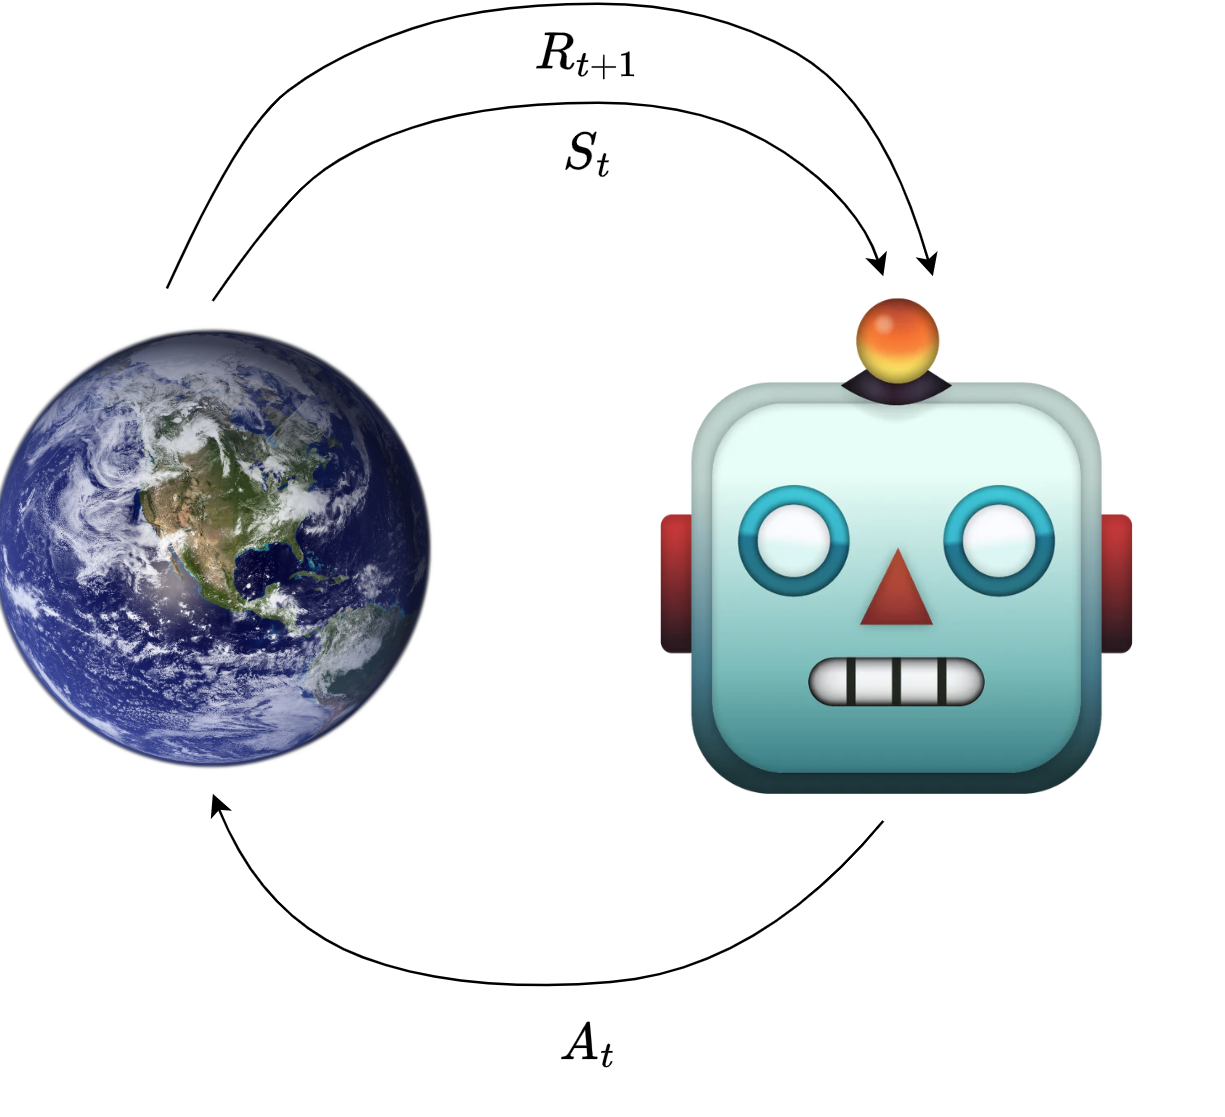
\includegraphics[width=\linewidth]{RLPL/images/MDP.png} \\[0.3em]
      {\small\textbf{Markov Decision Process}}
    \end{column}
  \end{columns}
\end{frame}

\begin{frame}{MDP Formulation}
  \begin{block}{State}
    Image features, model predictions, entropy (uncertainty).
    \begin{center}
      $\mathcal{S} = \{ \mathbf{X} ; \ \text{softmax}(\mathbf{y}) ; \ \mathcal{L}  \}$
    \end{center}
  \end{block}
  \begin{block}{Action}
    Assign pseudo-label or skip.
    \begin{center}
      $\mathcal{A} = \{ 0, \ldots, 9, ; \ \text{skip} \}$
    \end{center}
  \end{block}
  \begin{block}{Reward}
    Error Rate improvement of downstream model on validation data.
    \begin{center}
      $\mathcal R_{t} = -(e_{t} - e_{t-1})$
    \end{center}

  \end{block}
\end{frame}

%--------------------------

\section{Training Flow}
\begin{frame}{Workflow}
  \begin{enumerate}
    \item \textbf{Load} labeled and unlabeled MNIST data. \\~\\
    \item \textbf{Initiate} RL environment and agent.\\~\\
    \item RL agent selects \textbf{pseudo-label} actions. \\~\\
    \item \textbf{Retrain} downstream model with newly labeled data. \\~\\
    \item \textbf{Reward} is assigned based on downstream model's error rate.
  \end{enumerate}
\end{frame}

%--------------------------

\section{Project Setup}
\begin{frame}{Code Files}
  \begin{itemize}
    \item \textbf{main.py}: Entry point for training process.
    \item \textbf{env.py}: Custom RL environment handling pseudo-labeling episodes.
    \item \textbf{model.py}: Updates policy based on agent's actions for maximising reward.
    \item \textbf{utils.py}: Helper functions for data loading, metrics, etc.
  \end{itemize}
  \centering
  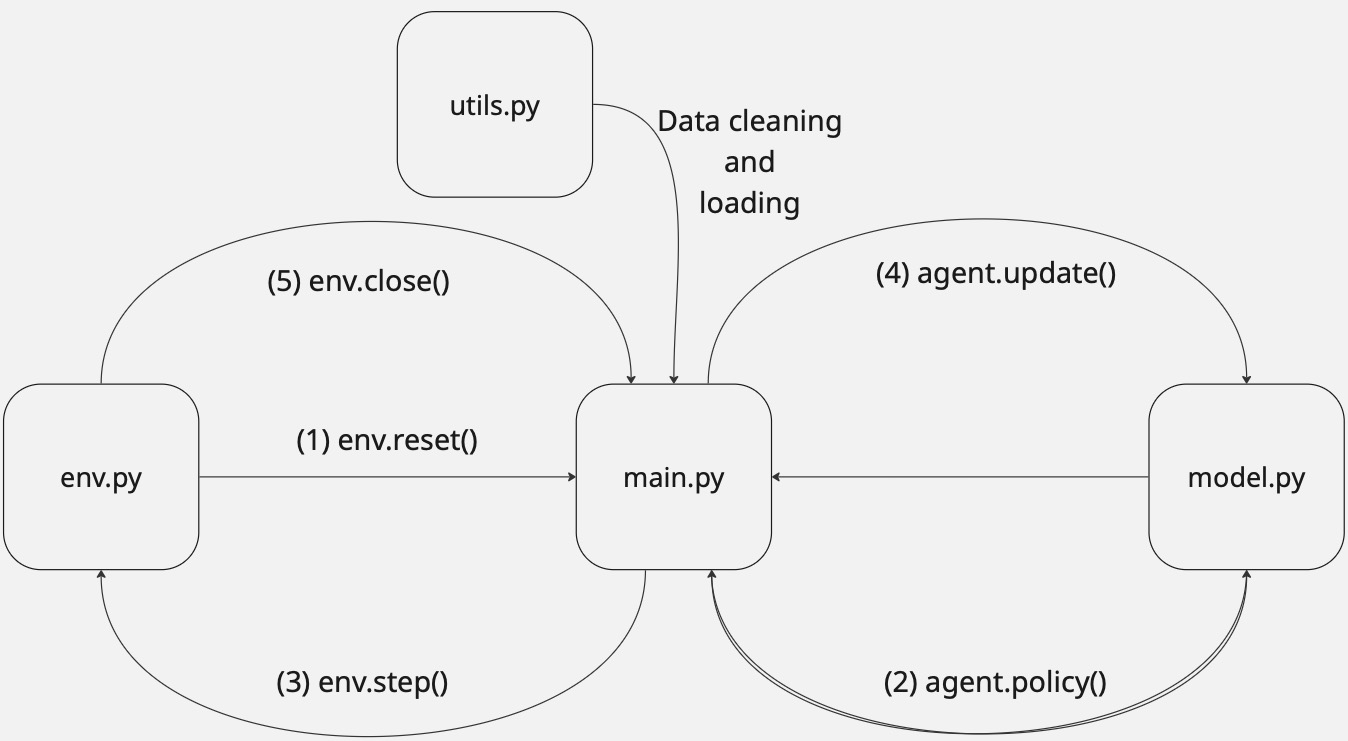
\includegraphics[width=0.7\linewidth]{RLPL/images/workflow.jpg} \\
\end{frame}

%--------------------------

\section{PseudoCode}
\begin{frame}{PseudoCode}
  \begin{algorithm}[H]
    \caption{RL agent training loop}
    \label{alg:rl_training_algpseudocode}
    \scriptsize
    \begin{algorithmic}
      \Require state\_dim, action\_dim, labeled\_data, unlabeled\_data, num\_episodes
      \State agent $\leftarrow$ \texttt{RLAgent}(state\_dim, action\_dim)
      \State env $\leftarrow$ \texttt{PseudoLabelEnv}(labeled\_data, unlabeled\_data) \\~\\
      \For{episode = 1 \textbf{to} num\_episodes}
      \State state $\leftarrow$ env.reset()
      \State done $\leftarrow$ false
      \While{not done}
      \State action $\leftarrow$ agent.select\_action(state)
      \State $(\text{next\_state},\ \text{reward},\ \text{terminated},\ \text{info}) \leftarrow \text{env.step(action)}$
      % \State agent.remember(state, action, reward, next\_state, done)
      \State state $\leftarrow$ next\_state
      \State done $\leftarrow$ terminated
      \EndWhile
      \State agent.update()
      \State accuracy $\leftarrow$ env.evaluate()
      \EndFor
      \State env.close()
    \end{algorithmic}
  \end{algorithm}
\end{frame}

%--------------------------

\section{Implementation Details}

\begin{frame}[fragile]{env.reset()}
  \begin{itemize}
      \lstinputlisting[basicstyle=\ttfamily\fontsize{5.5}{7.5}\selectfont,firstline=67, lastline=79]{RLPL/env.py} \\~\\
    \item \textbf{Input:} Random seed and options. \\~\\
    \item \textbf{Functionality:} Resets the environment. \\~\\ %by
      \begin{itemize}
          %\item resetting counters and rewards
          %\item shuffling unlabeled dataset
          %\item recalculating model's baseline accuracy on validation data
      \end{itemize}
    \item \textbf{Output:} Initial environment state and empty info dictionary.
  \end{itemize}
\end{frame}

\begin{frame}{model.policy()}
  \lstinputlisting[basicstyle=\ttfamily\fontsize{5.5}{7.5}\selectfont, firstline=73, lastline=73]{RLPL/model.py}
  \lstinputlisting[basicstyle=\ttfamily\fontsize{5.5}{7.5}\selectfont, firstline=82, lastline=88]{RLPL/model.py} \\~\\
  \begin{itemize}
    \item \textbf{Input:} Current state ($S_{t}$).\\~\\
    \item \textbf{Functionality:} Action (pseudolabel) is selected based on logits obtained from policy network. 
    \begin{center}
      $a \in \mathcal{A}(s)$
    \end{center} \\~\\
      \begin{itemize}
          %\item Converts the state to a tensor
          %\item passes it through the policy network to obtain logits
          %\item creates a categorical probability distribution, and samples one action from it.
      \end{itemize}
    \item \textbf{Output:} Selected action as integer.
  \end{itemize}
\end{frame}

\begin{frame}{env.step()}
  \lstinputlisting[basicstyle=\ttfamily\fontsize{5.5}{7.5}\selectfont, firstline=84, lastline=111]{RLPL/env.py}
\end{frame}

\begin{frame}[fragile]{env.step()}
  \begin{itemize}
    \item \textbf{Input:} Action selected by the agent.  \\~\\
    \item \textbf{Functionality:} There are multiple functionalities like: \\~\\
      \begin{itemize}
        \item Computes reward based on prediction and action.
        \item Updates pseudo-labeled data.
        \item Trains downstream model at episode end.
      \end{itemize} \\~\\
    \item \textbf{Output:} Returns next state, total reward, termination flag, and performance info (error rate, final reward).
  \end{itemize}
\end{frame}

\begin{frame}{model.update()}
  \lstinputlisting[basicstyle=\ttfamily\fontsize{5.5}{7.5}\selectfont, firstline=124, lastline=149]{RLPL/model.py}
\end{frame}

\begin{frame}[fragile]{model.update()}
  \begin{itemize}
    \item \textbf{Input:} Sampled states, actions, and rewards from agent experience. \\~\\
    \item \textbf{Functionality:} There are multiple functionalities like: \\~\\
      \begin{itemize}
        \item Computes advantages using rewards-to-go and value estimates.
        \item Updates policy network ($\pi_{\theta}(a|s)$) to maximize expected reward.
        \item Updates value network ($V^{\pi}_{\theta}$) to minimize prediction error.
      \end{itemize} \\~\\
    \item \textbf{Output:} Returns policy loss and value loss for performance tracking.
  \end{itemize}
\end{frame}

\begin{frame}{main.py (Bringing everything together)}
  \lstinputlisting[basicstyle=\ttfamily\fontsize{5.5}{7.5}\selectfont, firstline=6, lastline=28]{RLPL/main.py}
\end{frame}

%--------------------------

\section{Results and Insights}
\begin{frame}{Observations}
  \begin{itemize}
    \item Developed a functional custom Psuedo-Labeling environment.
    \item RL policy learns to prefer high-confidence samples.
    \item \textbf{Caveat:} Reward shaping has big impact on stability.
  \end{itemize}

  \begin{table}[h!]
    \centering
    \begin{tabular}{|l|c|}
      \hline
      \textbf{Model} & \textbf{Error Rate (\%)} \\
      \hline
      Random & 90.04 \\
      Downstream Model & 10.00 \\
      RLPseudolabelEnv & 8.00 \\
      \hline
    \end{tabular}
    \caption*{\textbf{Table 1.1} Comparison of Different Models}
  \end{table}

\end{frame}

%--------------------------

\section{Conclusion}
\begin{frame}{Conclusion}
  \begin{itemize}
    \item Demonstrated feasibility of RL-based pseudo-labeling. \\~\\
    \item Compared to naive pseudolabeling, RL improves selection. \\~\\
    \item Future work:
      \begin{itemize}
        \item To modify workflow for pseudo labeling in batches
        \item Test various reward functions
        \item Test the worflow with larger datasets
        \item Compare final RL approach with existing semi-suprvised techniques
      \end{itemize}
  \end{itemize}
\end{frame}

%--------------------------

\begin{frame}{Thank You}
  \centering
  \textbf{Questions?}
\end{frame}

\end{document}
